% !Mode:: "TeX:UTF-8"

\chapter{罗列、定理和代码环境使用方法}

\section{单层罗列环境}

天津大学学位论文一般可采用两种罗列环境:一种是并列条目有同样标签的~\verb|itemize|~罗列环境,另一种是具有自动排序编号符号的~\verb|enumerate|~罗列环境。这两种罗列环境的样式参数可参考图~\ref{fig:list}。
\begin{figure}[htbp]
\centering
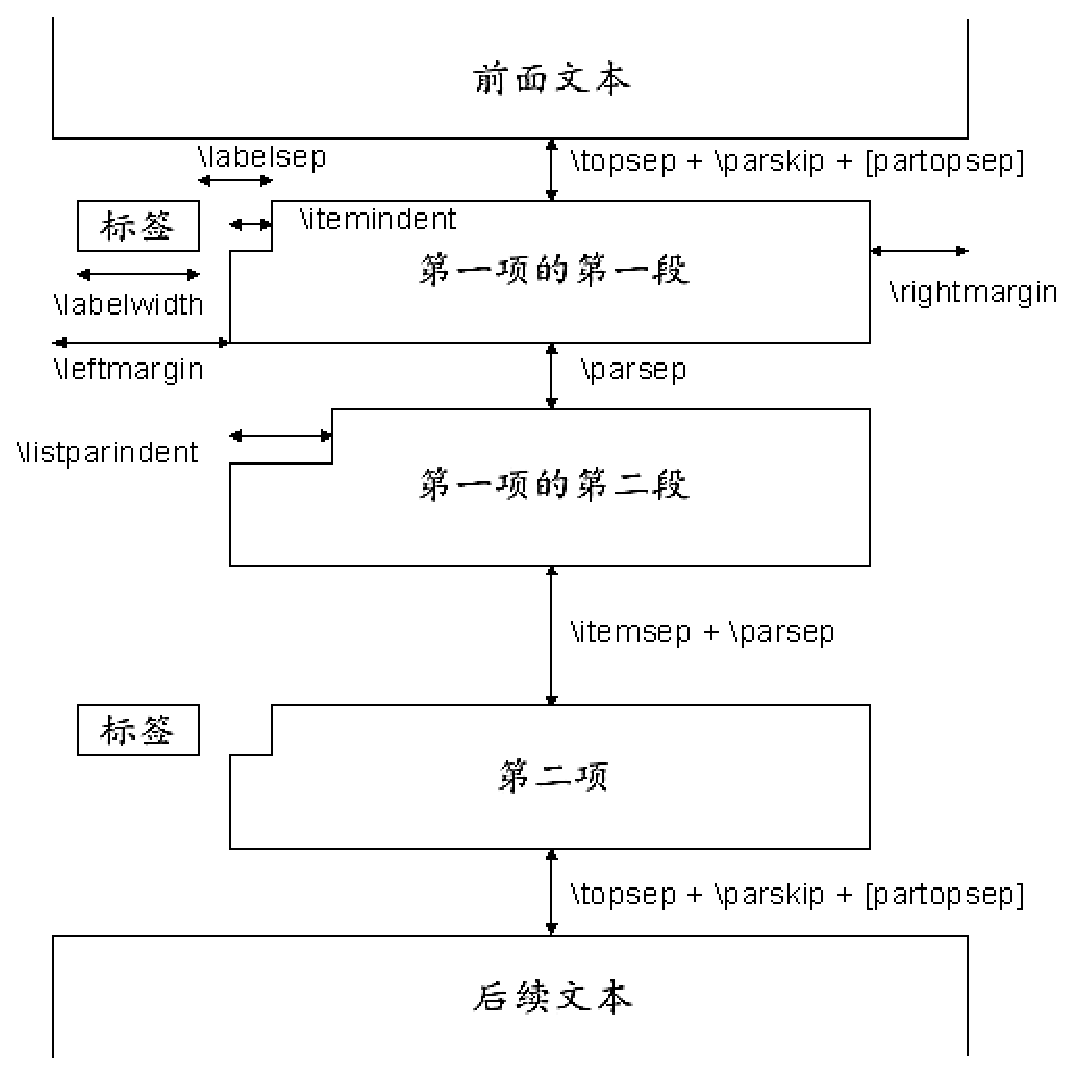
\includegraphics[width = 0.6\textwidth]{list}
\caption{罗列环境参数示意图}\label{fig:list}\vspace{-1em}
\end{figure}

通过调用~enumitem~宏包可以很方便地控制罗列环境的布局,其~format.tex~文件中的~\verb|\setitemize|~和~\verb|\setenumerate|~命令分别用来设置~\verb|itemize|~和~\verb|enumerate|~环境的样式参数。采用~\verb|itemize|~单层罗列环境的排版形式如下:

\begin{itemize}
\item 第一个条目文本内容
\item 第二个条目文本内容
\item 第三个条目文本内容
\end{itemize}

其代码如下

\begin{verbatim}
\begin{itemize}
  \item 第一个条目文本内容
  \item 第二个条目文本内容
  ...
  \item 第三个条目文本内容
\end{itemize}
\end{verbatim}

采用~\verb|enumerate|~单层罗列环境的排版形式如下:

\begin{enumerate}
\item 第一个条目文本内容
\item 第二个条目文本内容
\item 第三个条目文本内容
\end{enumerate}

其代码如下

\begin{verbatim}
\begin{enumerate}
  \item 第一个条目文本内容
  \item 第二个条目文本内容
  ...
  \item 第三个条目文本内容
\end{enumerate}
\end{verbatim}



\section{定理环境}

\begin{definition}[谱半径]\label{def:def1}
  称~$n$~阶方阵~$\mathbf{A}$~的全体特征值~$\lambda_1,\cdots,\lambda_n$~组成的集合为~$\mathbf{A}$~的谱,称
  $$\rho(\mathbf{A})=\max{\{|\lambda_1|,\cdots,|\lambda_n|\}}$$
\end{definition}
\begin{theorem}[相似充要条件]\label{lemma:l1}
  方阵$A$和$B$相似的充要条件是:~$A$~和~$B$~有全同的不变因子。
\end{theorem}
\begin{corollary}[推论1]\label{cor:cor1}
在赋范空间~$(X,\|\cdot\|)$~上定义~$d(x,y)=\|x-y\|$, 对任意~$x,y\in X$,~则~$(X,d)$~是距离空间。
\end{corollary}
\begin{proof}
  只需证明~$d(x,y)$~是距离。
\end{proof}
\newpage

定义代码如下:
\begin{verbatim}
 \begin{definition}[谱半径]\label{def:def1}
  称~$n$~阶方阵~$\mathbf{A}$~的全体特征值
  $\lambda_1,\cdots,\lambda_n$组成的集合为~$\mathbf{A}$~的谱,称
  $$\rho(\mathbf{A})=\max{\{|\lambda_1|,\cdots,|\lambda_n|\}}$$
\end{definition}
\end{verbatim}
\noindent\hrule

\vspace{0.1em}\noindent\hrule
\vspace{1em}
定理代码如下:
\begin{verbatim}
\begin{theorem}[相似充要条件]\label{lemma:l1}
  方阵$A$和$B$相似的充要条件是:$A$和$B$有全同的不变因子。
\end{theorem}
\end{verbatim}

\noindent\hrule\vspace{0.1em}

\noindent\hrule
\vspace{1em}
推论和证明代码如下:
\begin{verbatim}
\begin{corollary}[推论1]\label{cor:cor1}
在赋范空间~$(X,\|\cdot\|)$~上定义$d(x,y)=\|x-y\|$,
对任意$x,y\in X$,则$(X,d)$是距离空间。
\end{corollary}
\begin{proof}
  只需证明$d(x,y)$是距离。
\end{proof}
\end{verbatim}
\noindent\hrule\vspace{1em}

定理定义[]中是可选参数,用来说明定理的名称。其他环境格式书写与上面定理、定义、推论格式相同,可自己调用其他环境。
若需要书写定理定义等内容,而且带有顺序编号,需要采用如下环境。除了~\verb|proof|~环境之外,其余~9~个环境都可以有一个可选参数作为附加标题。

\begin{center}
\vspace{0.5em}\noindent\wuhao\begin{tabularx}{0.7\textwidth}{lX|lX}
定理 & \verb|theorem|~环境 & 定义 & \verb|definition|~环境 \\
例 & \verb|example|~环境 & 算法 & \verb|algorithm|~环境 \\
公理 & \verb|axiom|~环境 & 命题 & \verb|proposition|~环境 \\
引理 & \verb|lemma|~环境 & 推论 & \verb|corollary|~环境 \\
注解 & \verb|remark|~环境 & 证明 & \verb|proof|~环境 \\
\end{tabularx}
\end{center}
\section{代码环境}
很多和计算机专业背景相关的同学都会使用到代码环境,使用~\verb|\verb|~指令或者是~\verb|verbatim|~环境固然是一种选择,但是比不上专门的~lstlisting~环境这么专业。
\begin{lstlisting}
int main(int argc, char ** argv)
{
printf("Hello world!\n");
return 0;
}
\end{lstlisting}

\noindent\hrule
\vspace{0.1em}\noindent\hrule

\vspace{1em}

\noindent 代码如下:
\begin{verbatim}
\begin{lstlisting}
int main(int argc, char ** argv)
{
printf("Hello world!\n");
return 0;
}
\end{lstlisting}
\end{verbatim}
\noindent\hrule\vspace{1em}

在代码中显示的关键字为蓝色,框的左侧显示的是行号,这样便于读者阅读和查找代码,同时添加了浅蓝色的阴影边框,达到了美观的效果。
代码环境的设置已在~package~中~\verb|\lstset|~指令中定义。定义中支持跨页显示,可以将较长的代码置于~lstlisting~环境中。
\section{算法环境}
很多和计算机专业背景相关的同学会使用到算法环境,之前使用到的定理环境固然是一种选择,但是比不上专门的~algorithm2e~环境这么专业。为了实现专业和接近完美,本版本支持算法环境。如下所示:
\begin{algorithm}[H]
    \caption{算法标题}
    \label{alg:demoAlgo} % 贴上标签以便交叉引用
    \begin{algorithmic}[1]  % 这个 1 表示每一行都显示数字
    \STATE 初始化...
    \FOR{$i=0;i\le M; i\rightarrow i + 1$}
        \STATE 执行语句~1;
        \STATE 执行语句~2;
        \STATE ...
    \ENDFOR
    \STATE ...
    \WHILE{某条件}
        \STATE 执行语句~1;
        \STATE 执行语句~2;
        \STATE ...
    \ENDWHILE
    \STATE ...
    \end{algorithmic}
\end{algorithm}
\noindent\hrule
\vspace{0.1em}\noindent\hrule

\vspace{1em}

\noindent 代码如下:
\begin{verbatim}
  \begin{algorithm}[H]
    \caption{算法标题}
    \label{alg:demoAlgo} % 贴上标签以便交叉引用
    \begin{algorithmic}[1]  % 这个 1 表示每一行都显示数字
    \STATE 初始化...
    \FOR{$i=0;i\le M; i\rightarrow i + 1$}
        \STATE 执行语句~1;
        \STATE 执行语句~2;
        \STATE ...
    \ENDFOR
    \STATE ...
    \WHILE{某条件}
        \STATE 执行语句~1;
        \STATE 执行语句~2;
        \STATE ...
    \ENDWHILE
    \STATE ...
    \end{algorithmic}
\end{algorithm}
\end{verbatim}

